 \documentclass[twoside]{book}
\usepackage{geometry}
\usepackage{puzzles}



\geometry%{top=0.9in, bottom=0.9in,left=0.9in, right=0.9in, paperwidth=6in, paperheight=9in}
{top=0.9in, bottom=0.9in,inner=0.9in, outer=0.7in, paperwidth=6in, paperheight=9in}


\def\thetitle{Математические головочинки}
\def\theauthor{Питер Винклер}
\hypersetup{
pdftitle={\thetitle},
pdfauthor={\theauthor},
pdfsubject={Математика}}


\makeindex[title=Указатель головоломок,intoc]

\makeatletter
\newcommand{\rindex}[2][\imki@jobname]{%
  \index[#1]{\detokenize{#2}}%
}
\makeatother


\begin{document}
%\pagestyle{empty}

\title{\thetitle}
\author{\theauthor\\
\\
Перевод с английского большой компанией}
\date{}
\maketitle

\thispagestyle{empty}

Предварительное издание предназначенное исключительно для отлова ляпов. 

Исправления слать по адресу 
\url{petrunin@math.psu.edu}.

\vfill

\chapter{Разминка}


\setlength{\epigraphwidth}{.80\textwidth}
\epigraph{Мозг (сущ.) --- приспособление, которым думают, что думают.}{--- Амброз Бирс (1842---1914), Словарь Сатаны}

Начнём с нескольких довольно простых задач для разминки мозга.
Для них почти не потребуется математики, только чуть-чуть логики.

\subsection*{Половина роста}

В каком возрасте средний ребенок достигает половины роста, до которого он дорастёт когда вырастит?

\subsection*{Шарики в мешочках}

Сколько нужно шариков, чтобы разложить в 15 мешочков так,
чтобы во всех мешочках было разное число шариков?

\subsection*{Степени двойки}

Сколько людей составляют \emph{дважды две пары двойняшек}?

\subsection*{Катящийся карандаш}

Карандаш с пятиугольным сечением имеет надпись на одной из пяти граней.
Предположим карандаш катится по столу.
С какой вероятностью он остановится надписью вверх?

\subsection*{Портрет}

Посетитель указывает на портрет и спрашивает, кто это. 
«Братьев и сестер у меня нет,» --- отвечает хозяин, --- «но отец этого человека --- сын моего отца».
Кто изображен на картине?

\subsection*{Странная последовательность}

Каким должен быть следующий символ в этой последовательности?

\begin{figure}[h!]
\centering

\includegraphics[scale=0.5]{pics/ZYXW}
\end{figure}

\subsection*{Параметр языка}

Для испанского, русского или иврита он равен 1.
Для немецкого --- 7.
Для французского --- 14.
Чему он равен для английского?

\subsection*{Вниманию параскаведекатриафобов}

Правда ли, что 13-е число месяца выпадет на пятницу чаще,
чем на любой другой день недели,
или это только так кажется?

\medskip

Теперь задачи посерьезнее.

\subsection*{Честная игра}

Как сделать равновероятный выбор 50 на 50, подбрасывая гнутую монету?

\subsection*{Кривые на картофелинах}

Даны две картофелины.
Докажите, что на их поверхностях можно нарисовать по замкнутой кривой так, чтобы обе кривые были идентичны как кривые в трехмерном пространстве.

\medskip

Завершим размнику тремя вероятностными задачами; в них потребуется \emph{кое-что} вычислять.

\subsection*{Победа на Уимблдоне}

В результате временных магических способностей вы попали в финал ... на Уимблдоне и играете против Серены Уильямс или Роджера Федерера ...
Однако магия не работает до победы.
На каком счёте лучше всего отказаться от магии, чтобы максимизировать свои шансы одержать победу?

\subsection*{Макаронные циклы}

100 концов 50 сваренных длинных макаронин произвольно разбиты на пары и соединены вместе.
Сколько циклов вы ожидаете так получить в среднем?

\subsection*{Рулетка для ротозеев}

Элвин приехал в Лас-Вегас на математическую конференцию и оказался в казино.
У него есть немного времени перед докладом и 105 долларов в кармане.
Он подошёл к рулетке и увидел, что на колесе 38 чисел (0, 00 и от 1 до 36).
Если поставить 1 доллар на какое-то число, то выигрываешь с вероятностью 1/38, получая 36 долларов (взамен своего доллара, который в любом случае забирает казино).
В противном случае, он просто теряет свой доллар.

У Элвина достаточно времени ровно на 105 таких однодолларовых ставок, и он решает так и поступить.
Оцените вероятность того, что Элвин окажется в плюсе?
Скажем, превысит ли эта вероятность 10\%?

\section*{Решения и комментарии}

\subsubsection*{Половина роста}

Родители маленьких детей знают ответ: два года!
(То есть между вторым и третьим днями рождения.)
Да, человечек растёт очень нелинейно.

Задача предложена Джеффом Стейфом из Университета Чалмерса в Швеции.

\subsection*{Шарики в мешочках}

Потребуется четырнадцать шариков.
Положите пустой мешочек в мешочек с одним шариком, 
далее второй мешочек в третий, с ещё одним шариком, затем третий в четвертый, с ещё одним шариком, и так далее.
Таким образом в $i$-ом мешочке будет $i-1$ шарик (и $i-1$ мешков).

Если вы не догадались засовывать мешочки в мешочки, или подумали, что так не честно, то вам потребуется $0 + 1 \z+ \z\dots \z+ 14 \z= 15 \times 7 \z= 105$ шариков.

Задача предложена Диком Плотцем из Провиденса, штат Род-Айленд.

\subsection*{Степени двойки}

Ответ восемь.
Четвёрка слов «дважды», «две», «пары», и «двойняшкa» натакливает на мысль что должно получиться $2^4 \z= 16$ человек.
Но двойняшка это только один человек.

Классическая задачка.

\subsection*{Катящийся карандаш}

Мой коллега Лори Снелл подловил меня на этой задачке.
А вы попались?
Похоже, что ответ должен быть $\tfrac15$, но поскольку $5$ нечётно, карандаш будет лежать гранью вниз и ребром вверх.
Таким образом, ответ $0$ или, если хотите, $\tfrac25$, в зависимости от вашего толкования термина \emph{вверх}, но уж всяко не $\tfrac15$.

Эта головоломка приведена в провокационной книге Чамонта Ванга \cite{wang}.

\subsection*{Портрет}

Это древняя загадка;
она приводится в классической книге Рэймонда Смаллиана \cite{smullyan}.

«Сын моего отца» может означать только самого хозяина, поскольку у него нет ни братьев ни сестёр.
А значит на портрете сын хозяина.

\subsection*{Странная последовательность}

Эту загадку переслал мне Кит Кохон, юрист из Агентства по охране окружающей среды.
Это начало алфавита в обратном порядке, то есть ZYXW, но буква Z повернутой на 90° (вправо или влево), и каждая последующая буква повернута на дополнительные 90°.
Следующим символом, следовательно, должна быть повернутая буква V, то есть < или >.

\subsection*{Параметр языка}

Ответ семь (seven).
Этот любопытный загадочный вопрос был придуман Тиной Кэрролл, аспиранткой Технологического института Джорджии,
и он слегка математический. 
Каждое число это первое многосложное натуральное число в данном языке.

\begin{addedbytheeditors}
Наверно лучше оставить вопрос про русский язык и лучше добавить языков знакомых многим нашим людям --- наверно турецкий=2, грузинский и финский=1, японский=6...
\end{addedbytheeditors}


\subsection*{Вниманию параскаведекатриафобов}

Удивительно, но правда.
Насколько мне известно, это было обнаружено Банкрофтом Брауном (профессор математики в Дартмутском колледже, как и автор этих строк), который привёл свои расчёты в журнале American Mathematical Monthly \cite{brown}.
На это мне указал мой нынешней коллега Дана Уильямс.

Не трудно проверить, что в 688 из 4800 месяцев в 400-летнем цикле григорианского календаря 13-е число выпадает на пятницу.
Воскресенье и среда приходятся по 687, понедельник и вторник по 685, а четверг и суббота только по 684.
Для этого нужно помнить, что годы, кратные 100, не являются високосными, если только (как 2000 год) они не делятся на 400.

Происхождение суеверия относительно пятницы 13-го обычно связывается с датой приказа, отданного французским королем Филиппом IV (Филиппом Красивым), о разгроме ордена храмовников.

Потренировавшись, можно научиться определить день недели любой даты в истории, даже учитывая прошлые календарные сложности
(по крайней мере, если вы человек, подобный внушающему восхищение Джону Конвею из Принстонского университета).
Для более ленивых смертных, ориентированных на настоящее время, полезно помнить, что в любом году
04.04, 06.06, 08.08, 10.10, 12.12, 09.05, 05.09, 07.11, 11.07 и последний день февраля выпадают на один и тот же день недели.
(Это еще легче запомнить, если вы играете в крэпс ежедневно с 9 до 5.)
Этот день недели --- среда для 2007 года;
перед невисокосным годом он сдвигается на один, и на два перед високосным.

\subsection*{Честная игра}

Подбросьте гнутую монету дважды в надежде получить орёл и решку.
Если сначала выпадет орёл, назовём результат «ОРЁЛ»;
если сначала выпадет решка, назовите его «РЕШКА».
Если получим две решки или два орла, то придётся повторить.

Мне напомнил об этой головоломке Тамаш Ленгель из Маккалестерского колледжа;
её решение приписывается покойному великому математику и пионеру компьютерных наук Джону фон Нейману и иногда называется «трюком фон Неймана».
Оно основано на том, что даже если монета гнутая, последующие броски являются (или по крайней мере должны быть) независимыми событиями.
Конечно же придётся предположить, что гнутая монета может приземлиться на любую сторону!

Если вы хотите минимизировать количество бросков, чтобы принять решение, вышеупомянутую схему можно улучшить. Например, если вы получаете орёл-орёл при первой паре бросков и решка-решка при второй, то можно назвать результат «ОРЛОМ» (конечно же решка-решка, за которым следует орёл-орёл, должен быть «РЕШКОЙ»).
Возможны и другие улучшения.
Статья Шербана Наку и Ювала Переса \cite{nacu-peres} выдавливает последнюю каплю из минимизации ожидаемого количества бросков, независимо от вероятностей получения орла и решки.

Кстати сказать, в последние годы, вопрос извлечения честных случайных битов из различных ненадёжных случайных источников становится важным в теории вычислений и является предметом многих научных работ и существенных прорывов.

\subsection*{Кривые на картофелинах}

Рассмотрите пересечение картофелин!
Другими словами, представьте каждая картофелина это призрак и воткните одну в другую.
Пересечение их поверхностей образует кривую на каждой из них; их и следует нарисовать.

Эту милую головоломку можно найти (среди прочего) в книге \cite{berlekamp-rodgers}.

\begin{addedbytheeditors}
Несмотря на столь простое решение, точная математическая формулировка задачи остаётся не ясной.

Пересечение поверхностей картофелин может быть фракталом не содержащим замкнутых кривых даже если сами поверхности гладкие.
В случае если поверхности гладкие, картофелины легко расположить так чтобы пересечение было гладкой замкнутой кривой.
Тоже можно сделать и при более слабых предположениях.

Однако, без дополнительных предположений вопрос остаётся открытым \cite{agol};
то есть неизвестно \emph{содержат ли две произвольные вложенные сферы в евклидовом пространстве пару конгруэнтных замкнутых кривых?} 
Более того, похоже, что вопрос откыт даже если обе вложенные сферы имеют конечную площадь.
Это предположение кажется разумным; как заметил Пер Александерсон,
«Я стараюсь не брать картофель с бесконечной поверхностью --- его слишком долго чистить.»
\end{addedbytheeditors}

\subsection*{Победа на Уимблдоне}

Кажется очевидным, что следует ...
(Вероятно, вы предпочтёте подавать, но если ваша подача такая же, как моя, то может быть лучше чтобы подавал ваш противник...)

Но подождите, не так быстро!
Эти решения дают три шанса что вам повезёт и вы выиграете, но можно добиться шести шансов...

Амит Чакрабарти из Дартмутского университета предложил следующее улучшение, основанное на идее, что традиционно полный счёт теннисного матча включает игровые очки всех партий и, если ...
Тогда, например, вы могли бы ...
Теория здесь (признаю, что сомнительная), заключается в том, что пока вы находились под вашим магическим заклинанием, ваш противник ... и легче совершит ошибку ...

\subsection*{Макаронные циклы}

Эта старинная задача, переданна мне коллегой из Дартмутского колледжа, Даной Уильямс.
Она эквивалентна «Игре ???» на странице 198 в книге Мартина Гарднера \cite{gardner1971}.
Вам нужно вычислить вероятность создания цикла на каждом этапе.
Тогда, используя \emph{линейность матожидания}, можно будет заключить, что ожидаемое число циклов это сумма полученных вероятностей.

При соединении $i$-го конца, вы берёте конец цепи, и из оставшихся $101 - 2i$ концов, только один (другой конец этой цепи) приводит к циклу.
Следовательно, вероятность того, что ваше $i$-е соединение добавит цикл, равна $1/(101 - 2i)$, и, следовательно, ожидаемое общее число циклов равно $1/99 + 1/97 + 1/95 +\dots + 1/3 + 1/1 = 2{,}93777485\dots$; меньше трех циклов!

Если у нас $n$ макаронин и $n$ большое число, то матожидание числа циклов близко к половине $n$-го гармонического числа, что примерно равно половине натурального логарифма $n$.

\subsection*{Рулетка для ротозеев}

Я услышал эту историю от Элвина Берлекэмпа на конференции
«Gathering for Gardner VII».
Позже она появилась в замечательном разделе «Головоломки» журнала Emissary \cite{berlekamp-buhle}, весна/осень 2006 года.

Игра в рулетку очень выгодна для казино (американский вариант ещё выгодней европейского в котором нет двойного нуля).
Ясно, что если повторять невыгодную ставку достаточно долго, то обычно окажитесь в проигрыше.
Каждая однодолларовая ставка приносит средний убыток в  $1 - (1/38) \times 36 = 1/19$ доллара, то есть примерно в пять центов.

Однако 105 это не так уж много!
Эльвину достаточно выиграть три раза, чтобы оказаться в плюсе.
В этом случае он получит 108\$ за свои 105\$.
Вероятность того, что он никогда не выиграет, составляет $(37/38)^{105} \approx 0{,}0608$;
выиграет ровно раз, $105 \times (1/38) \times (37/38)^{104} \z\approx 0{,}1725$;
и два раза, $105 \times (104/2) \times (1/38)^2 \times (37/38)^{103} \approx 0{,}2425$.
Таким образом, вероятность оказаться в плюсе равна единице минус сумма этих трёх значений, что составляет $0{,}5242$ --- больше половины!

Конечно же это не означает, что Эльвин может дурачить Лас-Вегас.
Ведь когда ему не удается получить три победы, он теряет как минимум 33 доллара, намного больше, чем 3 доллара прибыли, которую он получает, когда выигрывает ровно три раза.
(А проигрывает он в 43\% случаев???)
В среднем Эльвин потеряет $105 \times (1/19) \approx 5{,}53$ долларов.

Рассмотрим более жёсткий вариант этой задачи.
Предположим, что у Эльвина есть 255\$, но ему нужно 256\$ чтобы зарегестрироваться на математической конференции.
Тогда лучше всего сделать ставку в 1\$, затем 2\$, затем 4\$, 8\$, 16\$, 32\$, 64\$ и, наконец, 128\$ на красное (или чёрное).
Первый раз, когда он выигрывает, он получает в два раза больше своей ставки и сразу же прекращает, имея ровно те 256\$, которые ему нужны.
Он терпит неудачу только если проигрывает все 8 ставок (и все свои деньги), что происходит с вероятностью только $(20/38)^8 < 0{,}006$.

Попробуйте сами если вам не страшно потерять 255\$.
Вы можете посетить казино и в 99\% случаев останетесь в плюсе.
Потом лучше бросить играть в азартные игры, очень рекомендую.

\chapter{Полёт фантазии}

%Кноп

\setlength{\epigraphwidth}{.80\textwidth}
\epigraph{Не стоит доверять глазам, когда разыгралось воображение.
}{--- Марк Твен (1835---1910), Янки при дворе короля Артура}

Следующие головоломки потребуют разработки \emph{плана},
и иногда вам придётся напрячь воображение!

\subsection*{Любовь в Клептопии}\rindex{Любовь в Клептопии}\label{Любовь в Клептопии}

Ян влюбился в Марию (по интернету), и он хочет послать ей обручальное кольцо.
Однако они живут в Клептопии, стране, где всё отправленное по почте будет неминуемо украдено, если только не отправлено в ящике, запертом на навесной замок.
У Яна и Марии много замков, но ни у кого из них нет ключа к замку другого.
Как им переслать кольцо?

\subsection*{Черви и вода}\rindex{Черви и вода}\label{Черви и вода}

Лори надоело, что черви забираются к ней на кровать.
Она поставила ножки кровати в вёдра с водой;
поскольку черви не умеют плавать, они не могут добраться до кровати по полу.
Однако теперь они ползут вверх по стенам и по потолку, и падают на кровать сверху.
Фу!

Как защититься от червей?

\parit{Примечания.}
Можно попробовать соорудить навесную конструкцию над кроватью.
Для того чтобы предотвратить падение червей на навес,
их дальнейшее проползание по навесу
и падение на кровать, возможно, стоит сделать жёлоб вокруг навеса и наполнить его водой.
Но ведь тогда черви смогут упасть на край жёлоба.
Хм...

\subsection*{Проверка страусиных яиц}\rindex{Проверка страусиных яиц}

В преддверии рекламной кампании страусиной ферме нужно проверить яйца своих страусов на прочность.
В мировой практике прочность определяют по самому высокому этажу Эмпайр-стейт-билдинга, с которого можно сбросить яйцо так, чтобы оно не разбилось.

Официальный инспектор фирмы, Оскар, понимает, что если он возьмёт с собой в Нью-Йорк одно яйцо,
то для определения прочности придётся (возможно) бросить его с \emph{каждого} из 102 %101???
этажей, начиная с первого.
А что если он возьмёт \emph{два} яйца?
Сколько бросков ему потребуется в худшем случае?

%\begin{addedbytheeditors}
%\textbf{Редакторам:}
%Тут возникает проблема с американской и русской нумерацией этажей + похоже, что Уинклер считает, что нет смысла бросать яйцо с нулевого этажа.
%\end{addedbytheeditors}


\subsection*{Опасная картина}\rindex{Ненадежная картина}

Требуется повесить картину за шнур, прикреплённый к раме.
Если это сделать, как обычно, перекинув шнур через два гвоздя (как показано на рисунке), и один из гвоздей выпадет, то картина останется висеть на другом гвозде (хотя и накренится).

Можно ли повесить картину так, чтобы она упала в случае, если выпадет \emph{любой} из двух гвоздей?

\begin{figure}[h!]
\centering
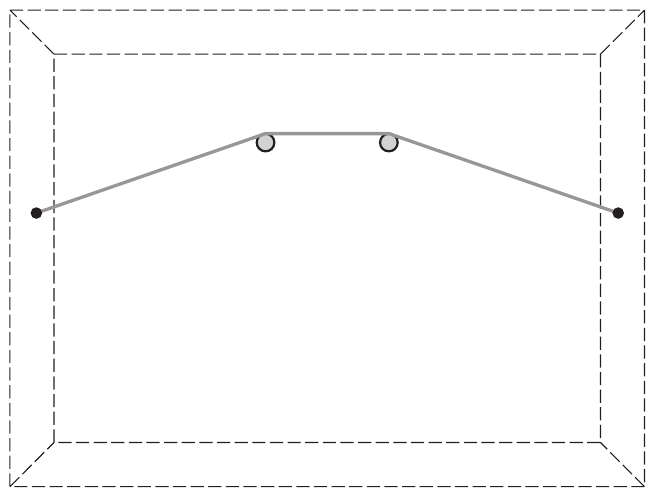
\includegraphics[scale=0.5]{pics/kartina1}
\caption{Эта картина останется висеть если выпадет любой из гвоздей.}
\label{pic:kartina1}
\end{figure}

\subsection*{Замок с дефектом}\rindex{Замок с дефектом}\label{Замок с дефектом}

Кодовый замок имеет три диска, с положениями пронумерованными от 1 до 8.
У замка есть дефект: чтобы его открыть, достаточно правильно выставить два числа из трёх.
Какое минимальное число (трёхзначных) комбинаций достаточно набрать, чтобы наверняка открыть замок?

\parit{Примечания.}
Есть много способов проделать это $64$-мя тестовыми комбинациями, например, можно перебрать все возможные варианты первых двух дисков или проверить все комбинации, сумма значений которых кратна 8.
Однако каждая тройная комбинация покрывает $22$ возможных случаев, а всего комбинаций $8^3 = 512$.
Поэтому в принципе могло бы хватить и $\lceil 512/22 \rceil = 24$ комбинаций.
То есть истина лежит где-то между $24$ и $64$; вопрос --- где?

\subsection*{Альтернативные кубики}\rindex{Альтернативные кубики}

 
Можно ли изготовить такую пару игральных кубиков, чтобы их суммы вели себя так же, как у пары обычных кубиков?
То есть должно быть два способа выбросить 3, шесть способов выбросить 7, один способ выбросить 12 и так далее.
У кубиков должно быть по шесть граней, и на каждой грани должно быть указано положительное целое число.

\subsection*{Совпадение монет}\rindex{Совпадение монет}

Сонни и Шер\footnote{Сонни и Шер --- популярный в 1970-е годы американский поп-рок дуэт Сонни Боно и его супруги Шер.\pr} играют в следующую игру.
В каждом раунде бросается честная монета.
Перед броском Сонни и Шер одновременно объявляют свои предположения о результате броска.
Они выигрывают раунд, если оба угадали правильно.
Требуется максимизировать долю выигранных раундов, предполагая, что игра идёт долго.

Пока что ответ очевиден --- 50\%: Сонни и Шер договариваются о последовательности предположений (например, всегда говорить «орёл»).
Очевидно, что лучшего им не добиться.

Однако перед началом игры игрокам сообщается, что Шер получит результаты всех бросков монеты заранее, прямо перед первым броском!
У неё есть возможность обсудить стратегию с Сонни заранее, но как только она получит данные о бросках, возможности передавать информацию больше не будет.
Возможно ли им добиться 70\%-й доли выигрышей?

\subsection*{Имена в ящиках}\rindex{Имена в ящиках}\label{Имена в ящиках}

Имена ста заключённых помещают в сто деревянных ящиков, по одному в каждом;
ящики расставляются в ряд на столе в комнате.
Заключённых приводят в комнату поочерёдно;
каждому позволяется заглянуть не более чем в 50 ящиков,
затем он должен покинуть комнату, оставив её в точно том же состоянии, как до прихода, и дальнейшее общение невозможно.

У заключённых есть возможность спланировать свою стратегию заранее, и им это понадобится --- если хотя бы один заключённый не найдёт своё имя, то казнят всех.
Найдите стратегию, вероятность успеха которой превысит 30\%.

\parit{Примечания.} Если каждый заключённый откроет случайный набор из 50 ящиков, то вероятность выжить составит незавидные
\[(\tfrac12)^{100}\z\sim 0{,}0000000000000000000000000000008.\]
Но они могут поступить и хуже --- если все откроют одни и те же 50 ящиков, то их шансы упадут до нуля.
Но тридцать процентов уж совсем недостижимы...
Очень хорошо --- вы поняли задачу!

\section*{Источники и решения}

\subsubsection*{Любовь в Клептопии}

Эта головоломка приводится в книге Саймона Сингха \cite{singh};
я узнал её от Кэролайн Калдербэнк, дочке пары математиков Ингрид Добеки и Роба Калдербэнка.
В решении Кэролайн, Ян отправляет Марии ящик с кольцом внутри, навесив на него один из своих замков.
По получении Мария навешивает свой собственный замок на ящик и отправляет её назад с обоими замками.
Когда Ян получает ящик, он снимает свой замок и отправляет ящик опять Марии; вуаля!

Это решение не просто игра;
на нём основан обмен ключами шифрования в протоколе Диффи — Хеллмана, историческим прорывом в криптографии.

В зависимости от предположений, возможны и другие решения.
Моё любимое было предложено компанией участников конференции
«Ga\-the\-ring for Gardner VII», включая оригамиста Роберта Лэнга.
Для этого Ян должен найти замок, ключ от которого имеет большое отверстие, или по крайней мере, отверстие, которое может быть достаточно увеличено сверлением, чтобы ключ мог быть нацеплен за дужку другого замка.
Ян использует этот второй замок, с упомянутым ключом на его дужке, чтобы запереть пустой ящичек, которую он отправляет Марии.
По прошествии времени, достаточном для пересылки (или возможно, после электронного подтверждения от Марии), он отправляет кольцо в другом ящике, запертой первым замком.
Когда Мария получает ящик с кольцом, она открывает её ключом, прикреплённым к первому ящичку, и получает кольцо.

\subsubsection*{Черви и вода}

Это скорее инженерная головоломка, чем математическая.
Она пришла ко мне от Балинта Вирага из Массачусетского технологического института.

Лори действительно может защититься от червей свесив с потолка большой навес, выходящий далеко за кровать.
Но навес должен загибаться внутрь под себя по краям, создавая кольцевой жёлоб, заполненный водой.
(Поперечный разрез навеса показан на рис. \ref{pic:chervi}.)

\begin{figure}[h!]
\centering
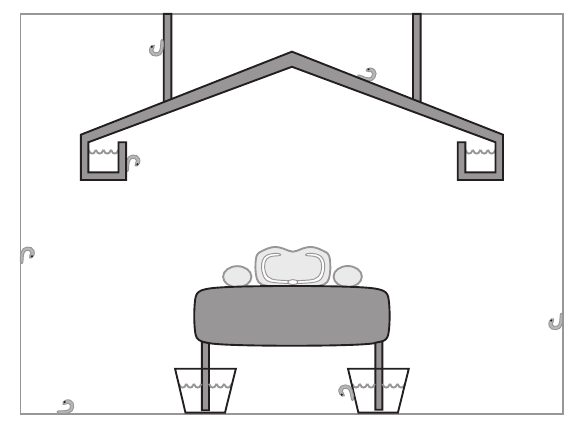
\includegraphics[scale=0.5]{pics/chervi}
\caption{Поперечный разрез Лори в защищённой от червей кровати.}
\label{pic:chervi}
\end{figure}

Если у червей нет способа проникнуть в спальню сверху, то Лори может защититься, обведя комнату по краю жёлобом с водой.

\subsubsection*{Инспекция страусиных яиц}

Вариант этой задачи появился в замечательной книге Джозефа Д. Э. Конхаузера, Дэна Веллемана и Стэна Уэгона \cite{konhauser-velleman-wagon}.

Часто полезно считать данное число (в нашем случае 102) переменной, даже если в конечном счёте нас интересует лишь одно значение.
Пусть $f(k)$ --- максимальное число этажей, которые можно проверить не более чем за $k$ бросков, имея вначале два яйца.
Таким образом, $f(1) = 1$ (прочность яйца может быть $0$ или $1$).
Предположим, что Оскару разрешено сделать $k$ бросков, и он делает первый с $n$-го этажа.
Если яйцо разбилось, то Оскару придётся бросить единственное оставшееся яйцо с 1-го этажа, затем с 2-го и так далее до $(n-1)$-го в худшем случае;
так что $n = k$ это наилучший вариант.
Если яйцо пережило падение с $k$-го этажа, то придётся проверить все этажи выше оставшимися $k-1$ броском (используя два яйца).
Следовательно, $f(k - 1) + k$ это максимальное число этажей, которые можно обработать,
и мы получили рекурсию $f(k) = f(k - 1) + k$.

Прямым вычислением получаем, что $f(2) = 3$, $f(3) = 6$, $f(5) = 10$ и так далее; в общем случае $f(k)$ равно сумме чисел от $1$ до $k$.
Поскольку таких чисел $k$, а их среднее равно $(k + 1)/2$, их сумма (иногда называемая «$k$-ым треугольным числом»), составляет $k(k + 1)/2$.
Первое значение $f(k)$, достигающее 102, это $f(14) = 14 \times 15/2 = 105$, то есть в худшем случае Оскару понадобится $14$ бросков.
Рекурсия указывает и на то как это сделать;
в нашем случае, трёхэтажный запас позволяет Оскару сбросить первое яйцо с одиннадцатого, двенадцатого, тринадцатого или четырнадцатого этажа.
Любой другой вариант может потребовать лишнего броска.

Давайте посмотрим, что происходит с тремя яйцами.
Определим $g(k)$ как максимальное число этажей, которые можно обработать $k$ бросками, начиная с трёх яиц.
Теперь Оскару нужно обработать $g(k \z- 1)$ этажей выше уровня первого броска, если яйцо переживёт падение;
или же $f(k - 1)$ этажей ниже этого уровня (тот же $f$, что и выше), потому что теперь у него лишь два яйца.
Получаем новую рекурсию: $g(k) = g(k-1) + 1 + (k - 1)k/2$, что даёт $g(2) = 3$ (пока без улучшений), но $g(3) = 7$.
В общем случае получаем $g(k)=k(k^2+5)/6$ и наименьшее значение $k$, для которого 
$g(k)\ge 102$, равно $9$.
То есть, если у Оскара есть три яйца,
то ему потребуется максимум девять бросков чтоб обработать Эмпайр-стейт-билдинг.

В общем случае, если $k$ велико, то число этажей, которые можно обработать, имея вначале $m$ яиц, равно $k^m/m!$ плюс члены низших порядков.
Отсюда следует, что с $m$ яйцами и небоскрёбом в $n$ этажей, где  $n$ намного больше $m$, число бросков, необходимых в худшем случае, будет около $(m!\times n)^{1/m}$.

\subsubsection*{Опасная картина}

Эту интересную головоломку предложил Джулио Дженовезе, аспирант в Дартмуте, который узнал её из нескольких источников в Европе.

Один из способов повесить картину изображён на рис. \ref{pic:kartina2}, с зазором, чтобы можно было в нём разобраться.
Шнур проходит над первым гвоздём,
далее идёт петля вокруг второго,
проходит опять над первым гвоздём, и затем снова петля вокруг второго гвоздя, но на этот раз с половинным поворотом.

\begin{figure}[h!]
\centering
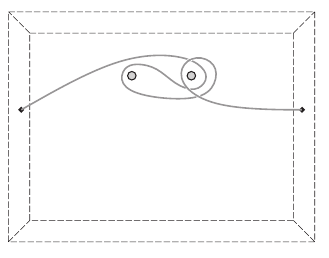
\includegraphics[scale=1]{pics/kartina2}
\caption{Эта картина упадёт если выскочит любой из двух гвоздей.}
\label{pic:kartina2}
\end{figure}

Существуют также некоторые нетопологические решения: например, можно сдавить петлю между двумя близко расположенными гвоздями, предполагая, что ширина головки гвоздя не намного больше толщины шнура.
Но зачем полагаться на трение, когда можно использовать математику?

\begin{addedbytheeditors}
Попробуйте повесить картину на $n$ гвоздей так, чтобы она упала если выскочит любой из них.
А можно ли повесить так, чтоб картина осталась висеть при выпадании одного гвоздя, но падала при выпадании двух?
Хороший обзор подобных задач дан в \cite{demaine2014}, но он не включает результата из \cite{gartside-greenwood}, дающего наилучий способ решения задачи с $n$ гвоздями (без заузливания шнура).
\end{addedbytheeditors}

\subsubsection*{Дефективный кодовый замок}

Этот шедевр комбинаторики достался мне от Амит Чакрабарти из Дартмута;
он был предложен Восточной Германией для Международную математическую олимпиаду 1988 года.

Задачи такого рода лучше решать геометрически.
Пространство всех комбинаций представляет собой комбинаторный куб $8 \times 8 \times 8$.
Каждый раз, когда мы проверяем точку куба, мы вычёркиваем все точки на трёх её координатных линиях.

Представив задачу таким способом, должно быть видно, что лучший способ вычеркнуть все точки это брать все тестовые точки в двух противоположных осьмушках $4 \times 4 \times 4$ нашего куба.
Так можно догадаться до следующего решения.

Давайте проверим все комбинации с числами из $\{1, 2, 3, 4\}$, сумма которых кратна $4$.
Их всего шестнадцать, так как если вы выбираете числа на первых двух (или любых двух) дисках, то число на третьем определяется однозначно.
Теперь попробуем те же комбинации, добавив $(4,4,4)$, то есть, добавив $4$ к каждому из трёх чисел;
их ещё $16$, и мы утверждаем, что вместе эти $32$ комбинации вычёркивают все.

Проверка довольно лёгкая.
Правильная комбинация должна иметь либо два (или более) числа из $\{1, 2, 3, 4\}$, либо два или более числа из  $\{5, 6, 7, 8\}$.
В первом случае положение третьего диска единственно (это число в правильной комбинации может не входить в $\{1, 2, 3, 4\}$), так что получена тройка среди первых $16$ тестовых комбинаций.
Второй случай аналогичен.

А вот способ Амита (есть и другие), объясняющий, что нельзя обойтись $31$-й или менее тестовой комбинацией.
Предположим, что $S$ --- это покрытие, и $|S| = 31$.
Пусть $S_i = \{\,(x, y, z) \z\in S : z = i\,\}$ будет $i$-м уровнем $S$.

Рассмотрим три множества:
$A=\{1, 2, 3\}$,
$B = \{4, 5, 6, 7, 8\}$,
и $C \z= \{2, 3, 4, 5, 6, 7, 8\}$.
По крайней мере, один уровень $S$ должен содержать три или меньше точек;
можно считать, что это $S_1$, и $|S_1| = 3$.
(Если $|S_1| \le 2$, то дойти до противоречия ещё проще.)
Точки $S_1$ должны лежать в некотором $3 \times 3 \times 1$ подкубе;
можно считать, что они лежат в $A \times A \times {1}$.

Заметим, что $25$ точек в $B \times B \times \{0\}$ должны быть вычеркнуты точками, не входящими в $S_1$.
Никакие две из них не могут быть вычеркнуты одной точкой в $S$.
Следовательно, $S - S_1$ содержит подмножество $T$ размером $25$, которое лежит в подкубе $B \times B \times C$.
Теперь рассмотрим множество $P = \{\,(x, y, z) : z \in C, (x, y, 1) \notin S_1 , (x, y) \notin B \times B\,\}$.
Легко подсчитать, что $|P| = (64-3-25) \times 7 = 252$.
Точки в $P$ не вычёркиваются $S_1$, и каждая точка в $T$ может вычеркнуть не более $3 + 3 = 6$ точек в $P$. Следовательно, есть по крайней мере $252 - 6 \times 25 = 102$ точки в $P$, которые должны быть вычеркнуты точками в $S - S_1 - T$.

Однако осталось всего $|S - S_1 - T | = 31 - 3 - 25 = 3$ тестовых точек, и каждая из них вычёркивает ровно $22$ точки.
Поскольку $22 \times 3 = 66 \z< 102$, приходим к противоречию. 

\subsubsection*{Альтернативные кубики}

Эта задача настолько известна, что у её решение есть имя: «кубики Шихермана».
В заметке Мартина Гарднера 1978 года \cite{gardner1978} или в ego книге \cite{gardner1989} можно узнать об их открытии полковником Джорджем Шихерманом, сейчас проживающим в Уэйсайд, Нью-Джерси.
Единственная пара кубиков Шихермана имеет метки $\{1, 3, 4, 5, 6, 8\}$ и $\{1, 2, 2, 3, 3, 4\}$.

Возможно, вы нашли ответ перебором, и это вполне подходящий способ решения.
Однако есть и другой способ, иллюстрирующий мощный математический инструмент --- \emph{производящие функции}.

Идея в том, чтоб сопоставить кубику многочлен от переменной $x$, в котором коэффициент при $x^k$ равен числу граней кубика с меткой $k$.
Обычный кубик, например, будет соответствовать многочлену $f(x) = x \z+ x^2 \z+ x^3 \z+ x^4 \z+ x^5 \z+ x^6$.

Ключевое наблюдение заключается в том, что результат броска двух (или более) кубиков представлен произведением их многочленов.
Например, если мы бросаем два обычных кубика, то коэффициент $x^{10}$ в произведении (то есть в $f(x)^2$) есть число способов выбора двух членов из $f(x)$, произведение которых равно $x^{10}$ ---
это $x^4 \times x^6$, $x^5 \times x^5$ и $x^6 \times x^4$; они представляют три способа получить сумму $10$.

Следовательно, если $g(x)$ и $h(x)$ --- многочлены наших кубиков, то $g(x) \times h(x) = f(x)^2$.
Многочлены, как и числа, единственным способом разлагаются на простые сомножители;
многочлен $f(x)$ разлагается как $x(x + 1)(x^2 + x + 1)(x^2 - x + 1)$.
Чтобы получить произведение $g(x)$ и $h(x)$ равное $f(x)^2$, нам нужно взять каждый из этих $4$ сомножителей и добавить по одной его копии в $g(x)$ и в $h(x)$, или же две его копии в один либо в другой.
Но есть следующие ограничения:
в полученных многочленах $g(x)$ и $h(x)$ не может быть свободных членов (это бы означало, что некоторые стороны помечены нулём);
не допускаются отрицательные коэффициенты;
также сумма коэффициентов в каждом из этих многочленов должна равняться 6.


Единственный решение (кроме $g(x) = h(x) = f(x)$) это
\[g(x)
=
x(x + 1)(x^2 + x + 1)
=
x + 2x^2 + 2x^3 + x^4\]
и
\[h(x)
=
x(x + 1)(x^2 + x + 1)(x^2 - x + 1)^2
=
x + x^3 + x^4 + x^5 + x^6 + x^8,\]
или наоборот.

Мы всё ещё использовали перебор, но таким методом можно решать задачи посложнее.
Во-первых, можно придумать альтернативы для пары восьмигранных игральных костей, пронумерованных от $1$ до $8$ (есть три альтернативных варианта), или для бросания трёх обычных кубиков (много способов).

Читателям, которые хотят поглубже изучить эту тему, стоит обратиться к отличной статье Джо Галлиана и Дейва Русина \cite{gallian-rusin}.

\subsubsection*{Совпадение монет}

Эту задачу предложил мне Одед Регев, из Техниона, в Израиле.
Сонни и Шер могут выиграть более чем в 2/3 случаев.
Для этого разделим последовательность бросков на блоки по три.
Перед каждым блоком Шер \emph{оповещает} Сонни, будут ли в следующем блоке в основном орлы или решки;
если первое, Сонни говорит «ООО» в этом блоке; если второе, то «РРР».

Но как Шер передать эту информацию?
Чаще всего Сонни ошибается (в точности) раз в блоке.
Перед этим броском Шер говорит «О», сообщая, что в следующем блоке будут в основном орлы, и «Р» в противном случае.
Для двух других бросков в текущей тройке Шер даёт правильный ответ (вместе с Сонни), гарантируя две из трёх побед.
Если случится, что Сонни может угадать все три броска в текущей тройке,
то один раз --- скажем на последнем броске, Шер действует, как описано выше, даже если это стоит им потери одной победы.
Таким образом, после первого блока Сонни и Шер будут набирать две победы из трёх, когда блок состоит из двух орлов и одной решки или двух решек и одного орла.
Когда блок состоит полностью из орлов или полностью из решек (что происходит с вероятностью 1/4), они получают две победы из трёх в половине случаев и три из трёх в остальной половине.
Значит доля успеха составит $3/4 \times 2/3 + 1/4 \times 5/6 = 17/24 > 70.8\%$.
Обратите внимание, что даже в наихудшем случае (например, если последовательные орлы и решки выбираются противником, а не случайны) этот метод гарантирует долю успеха хотя бы $2/3$.

Оливье Госснер, Пенелопа Эрнандес и Абрахам Нейман \cite{gossner} доказали, что с более сложными версиями этой схемы Сонни и Шер могут приблизиться к любой доле успеха равной $x$, где $x$ --- единственное решение уравнения
\[-x \log_2 x - (1 - x) \log_2 (1 - x) + (1 - x) \log_2 3 = 1,\]
и лучшего добиться нельзя.
Более того, это утверждение остаётся верным независимо от того, случайны ли броски монеты или нет!
Поскольку это значение $x$ составляет около $0{,}8016$, Сонни и Шер могут на самом деле добиться победы более чем в $80\%$ случаев, даже если оппонент играет против них.

\subsubsection*{Имена в ящиках}

У этой головоломки короткая, но увлекательная история.
Она придумана датским специалистом по информатике Петером Бро Милтерсеном;
её версия появилась в завоевавший широкое признание статье, написанной им и Анной Галь \cite{gal-miltersen}.
Однако Милтерсен не знал  решения, пока его коллега Свен Скиум не указал ему на это во время обеда.
В конечном итоге головоломка дошла до меня (в несколько усложнённой форме) через Дорит Ахаронов.

Чтобы её решить, заключённые должны сначала договориться о случайном соответствии ящиков со своими именами.
(Это сделает невозможным разложить имена в ящиках так, чтобы помешать протоколу, описанному ниже.)
Попадая в комнату, каждый заключённый проверяет свой собственный ящик (то есть ящик, с которому соответствует его имя).
Затем он заглядывает в ящик, соответствующий имени, которое он только что нашёл,
затем в ящик, соответствующий имени, найденному во втором ящике, и так далее, пока он не найдёт своё собственное имя или не откроет 50 ящиков.

Вот такая стратегия, но почему она работает?
Соответствие, между именем владельца ящика и именем, найденном в его ящике, представляет собой перестановку из 100 имён, выбранную равномерно случайным образом из набора всех таких перестановок.
Каждый заключённый идёт по циклу перестановки, начиная со своего имени.
Если цикл не длиннее 50, то он находит своё имя.
Если перестановка не длинней 50, то это сработает для всех, и заключённые будут спасены.

Вероятность того, что равномерно случайная перестановка чисел от $1$ до $2n$ не содержит ни одного цикла длиной более $n$, равна по крайней мере, $1$ минус натуральный логарифм от $2$, что составляет около $30,6853\%$.

Чтобы увидеть это, положим $n < k \le 2n$ и сосчитаем перестановки, имеющие цикл $C$ длиной ровно $k$.
Есть $\binom{2n}k$ способов выбрать имена в этом цикле, $(k - 1)!$ способов упорядочить их в $C$
и $(2n - k)!$ вариантов перестановки остальных имён;
произведение этих чисел равно $(2n)!/k$.
Поскольку в данной перестановке не более одного $k$-цикла, вероятность того, что такой имеется, в точности равна $1/k$.
Значит вероятность отсутствия длинного цикла равна
\[1-\frac{1}{n}-\frac{1}{n+1}-\dots-\frac{1}{2n}=1-H_{2n}-H_n\]
где $H_m$ --- сумма обратных чисел первых $m$ положительных целых чисел, что приблизительно равно $\ln m$.
Таким образом, наша вероятность будет близка к $1 - \ln 2n + \ln n = 1 - \ln 2$, на самом деле всегда чуть больше этого значения.
Для $n = 50$ мы получаем, что заключённые выживают с вероятностью $31,1827821\%$.
Недавно Юджин  Кертин и Макс Варшауэр \cite{curtin-warshaue} показали, что это решение нельзя улучшить.

Ламберт Брайт и Рори Ларсон, а также независимо Ричард Стэнли из Массачусетского технологического института, предложили следующую вариацию.
Предположим, что каждый заключённый должен заглянуть в \emph{не менее} чем 50 ящиков, и требование для выживания заключается в том, чтобы каждый заключённый \emph{не} нашёл собственное имя?
Несмотря на то, что цель полностью противоположна, похоже, что у заключённых нету лучшего варианта чем как следовать точно той же стратегии.
Однако теперь они выживают лишь, если каждый цикл длиннее $50$, а это происходит только при наличии единственного большого цикла длины $100$ --- шансы составляют ровно $1$ к $100$.
Не очень обнадёживает, но всё же лучше, чем $1$ к $2^{100}$.

Заметим, что у заключённых будут те же шансы, если каждому потребуется заглянуть в $99$ ящиков --- снова они следуют стратегии и выигрывают если случайная перестановка является циклом.
В этом случае сразу очевидно, что лучшей стратегии нет.
Ведь самый первый заключённый, чтобы он не делал, выживет с вероятностью $1\%$.
Забавно, что, если следовать этой стратегии, то как только повезло первому заключённому, так автоматически везёт всем остальным!


{
\small

\printindex

}

{

\sloppy

\printbibliography[heading=bibintoc]


\fussy

}

\newpage

{

\tableofcontents

}

\end{document}
